\section{Discussion}

\subsection{Answering Research Questions}

\begin{paraphrase}
 \subsubsection{RQ1}
Do the popular DFR tools meet the NIST CFTT expectation? 
If not, which tool meets which part of the expectation? 

Generally, we found that the DFR tools we tested did not consistently meet the NIST CFTT expectation.
TestDisk failed to fulfill core feature 1 because it did not identify deleted files in two test cases.
All tools fulfilled core feature 2, as they produced a recovered object for every deleted file they identified.
Autopsy and Magnet AXIOM failed to fulfill core feature 3 because in several test cases they did not recover data they had access to.
All tools failed to fulfill core feature 4 because in many cases they recovered data which was not part of the original file.

\subsubsection{RQ2}
What factors make the tools fail or succeed?

The most common factor causing tools to fail is when a deleted file has been overwritten.
Core feature 4 requires that a tool only recover data which was originally a part of the deleted file.
A tool's success regarding this feature is thus a measure of its restraint.
The only tool to consistently fulfill core feature 4 is FTK Imager.
When it detects that a file has been partially or completely overwritten by another file, it omits the deleted sections (and everything after them in FAT).
However, in cases when the overwriting file has also been deleted, even FTK fails to fulfill this core feature.
It is worth noting that Autopsy does appear to react to overwritten files; for some cases of overwriting in FAT, it returns only a single cluster, presumably the starting cluster of the deleted file.
However, since that cluster has been overwritten, Autopsy still fails to fulfill core feature 4 in those cases.

Another factor that causes multiple failures is simulated in FAT cases 8, 9, and 10.
In FAT, a file can be written starting close to the end of the file system, without enough space to fit contiguously.
In such cases, the file must be fragmented, and since it is already at the end of the file system, the second fragment will appear closer to the beginning of the file system (this is illustrated in Figure \ref{fig:case_8}).
This scenario could realistically occur when the file system is almost full.
In these cases, no tool is able to recover the second fragment of the deleted file; however, because FAT fragmentation is unpredictable, we only require them to recover the first fragment.
Interestingly, Autopsy and Magnet AXIOM fail to recover anything at all, with Autopsy returning a short file of null data, and Magnet AXIOM returning an empty file after displaying an error message.
\end{paraphrase}

\subsubsection{RQ3}

\TODO{TODO}

\subsubsection{RQ4}

\TODO{TODO}


% \subsection{Hybrid Tools} probably just cover this in the approach section

\subsection{Ambiguity in NIST Guidelines}
% Metadata
\subsubsection{FAT Fragmentation and Metadata-Based Tools}
\begin{paraphrase}
Core feature 3's requirement that a tool recover ``all non-allocated data blocks identified in a residual metadata entry''\cite{meta:dfr:standards} is not well-defined when considering a FAT file system. 
In FAT, the only relevant metadata left over after file deletion is the address of the first cluster of file data, and the file's length. 
If the deleted file is fragmented at any point, no evidence remains in the metadata. 
Therefore, interpreting the wording very closely, a tool is only required to recover the first cluster of a file's data. 
As this would not be particularly useful, it is unlikely that this was the intended meaning. 
For these tests we interpret core feature 3 as requiring the first contiguous segment of unallocated clusters starting from the first cluster originally allocated to the deleted file. 
In other words, if the file is fragmented, the tool must recover at least the first fragment. 
If a file is partially overwritten, the tool must recover at least the clusters before the overwritten part.
In essence, the tool is only required to recover data for which it does not have to guess what file the data belongs to.
However, it should be emphasized this is an assumption and the intent of the standard in this case needs clarification.
\end{paraphrase}

\subsubsection{Contradictory Core Features for Metadata-Based Tools}
\begin{paraphrase}
When designing test cases, we found situations in which core features 3 and 4 are entirely incompatible. 
Core feature 3 specifies ``all non-allocated data blocks identified in a residual metadata entry,''\cite{meta:dfr:standards} but that can sometimes still include data from other files. 
One such situation is when a deleted file is overwritten, and then the overwriting file is also deleted, such as in case 5i (as seen in Figure \ref{fig:case_5i}).

% \begin{figure}[h]
%     \centering
%     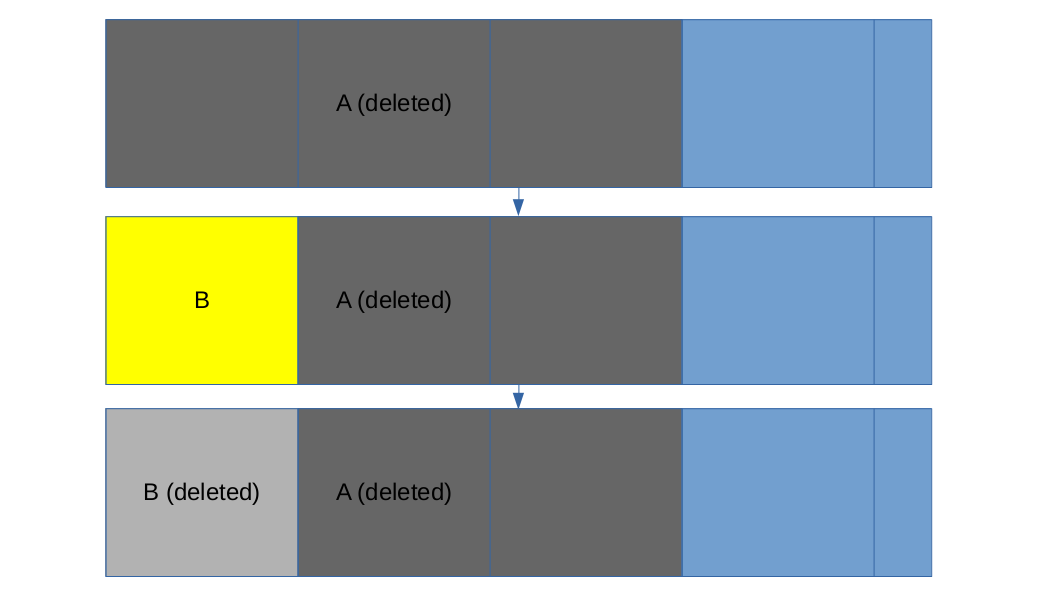
\includegraphics[width=\linewidth]{fig/case5i.png}
%     \caption{Test Case 5i}
%     \label{fig:case_5i}
% \end{figure}

Assuming the file system is NTFS (to avoid the aforementioned ambiguity with core feature 3 and FAT), the residual metadata entry for File A (in this case its Master File Table entry) should list every cluster File A once occupied. 
All of those clusters are unallocated, so to fulfill core feature 3, the tool must recover them. 
However, some of those clusters have been overwritten by File B. Core feature 4 requires that a tool only recover ``data blocks from the Deleted Block Pool,''~\cite{meta:dfr:standards} and defines the Deleted Block Pool as all blocks which ``have not been reallocated or reused.''~\cite{meta:dfr:standards}
Core feature 3 would require tools to recover the clusters reused by File B, while core feature 4 would forbid this. 
It could be argued that the tool should use File B's metadata to recognize that File B overwrote File A, but this is not always realistic. 
While the file system stores information such as creation and modification times, this is not ``essential metadata,'' meaning it is not involved in the operation of the file system, so operating systems may implement it inconsistently, or not at all.~\cite{carrier:filesystems}
Since the time information cannot be counted on to be reliable, there is no way to know for sure which file overwrote which. 
It is also possible for File B's metadata entry to be overwritten at some point before File A's, in which event there is no way for the tool to know File B even existed.

The standards document acknowledges that the ``potential for corruption [is] inherent with data that is no longer maintained by a file system,''~\cite{meta:dfr:standards} and that the recovered object ``may not completely match the original FS-Object.''~\cite{meta:dfr:standards}
We propose the standards themselves should be revised to better account for such situations.
This could mean adding an exception to either the third or fourth core feature, for cases in which data blocks are overwritten and subsequently deallocated.

NIST's James Lyle proposes that rather than deal with the complications involved in accommodating 
many different file systems, standards should be written for ``an ideal file system that leaves in 
residual metadata  all  information  required  to  reconstruct  a  deleted  file''~\cite{lyle2011-ICDF2C}. 
While this can result in tools being held to an impossible standard when using certain file systems, 
Lyle says that is acceptable because the user experience will be the same regardless of whether a feature is impossible or has merely been left out.
If the NIST guidelines were created with such an ideal file system in mind, the current standards may be adequate.
However, that philosophy should be clarified in the guidelines document to avoid confusion.
\end{paraphrase}



% Carving
\subsubsection{False-Positives from File Carving}
% What to do about additional files? It's clear for CR1, but not for the others.
\TODO{still need to write a lead-in to this}

 
Interpreting ``each carved file'' to include even the ones with no relation to the original files results in dramatically low scores for tools like Scalpel (which carved at least 50 additional ``files'' from most of our test images), while favoring tools which are more conservative in their recovery.
However, this would would obscure a relevant trade-off, that a more aggressive tool will have a high false-positive rate, but may recover files that a more conservative tool would miss.
An investigator may have this trade-off in mind when selecting a DFR tool, so the NIST guidelines should not make a tool that lies on one side of that trade-off look objectively worse than others.
As the standards are currently written, a tool that carves only one file from an image, but recovers it correctly, would be considered perfect on four out of five core features.
Meanwhile, a tool that perfectly carves all 40 files from an image, but also returns 100 false-positives, would likely score very poorly for core features 3, 4, and 5.
It would score especially poorly on core feature 5 as false-positives will almost never be a valid file.
Since the NIST guidelines do not directly account for the false-positive rate, it indirectly and disproportionately affects several core features, diluting their usefulness.

To resolve this issue, we propose the following changes to the NIST guidelines:
\begin{arabiclist}
 \item Add a new definition: \emph{Positive Carved File}, a carved file which corresponds to a supported file header signature from a source file that is present in the search arena. \TODO{come up with a better name for this}
 \item In core features 3, 4, and 5, change ``carved file'' to ``positive carved file.''
 \item Add an additional core feature: \emph{The tool shall not return any carved files that do not correspond to a supported file header signature from a source file that is present in the search arena.} This could be scored as the ratio of positive carved files to total carved files.
\end{arabiclist}

The intent of these changes is to somewhat atomize the guidelines, so each core feature evaluates a tool on a single capability.
This should make the trade-offs of certain tools more apparent, enabling investigators to make more informed and nuanced tool choices based on the capabilities that are most important for their use case.

\subsection{Related Work}

\begin{paraphrase}
 Arthur et al. published an article~\cite{arthur2004} in 2004 which analyzes several DF (digital forensics) tools, including FTK Imager.
While the tools are judged based in part on file recovery capabilities, the article does not present how these judgments were reached.
The article also addresses DF tools' disk imaging and hashing functionalities.

James Lyle from NIST published an article~\cite{lyle2011-ICDF2C} in 2011, which lays out a strategy to evaluate the metadata-based DFR tools. To the best of our knowledge, 
his is one of the first works that identified some of the challenges in setting standards for evaluation of metadata-based DFR tools.
In our understanding, NIST considered the above findings~\cite{lyle2011-ICDF2C} while they set the guidelines for metadata-based DFR tools.  
The NIST guidelines~\cite{meta:dfr:standards} are publicly available on the NIST CFTT portal~\cite{cftt:nist}, which we have used in the current work.

Recently, Loja et al.~\cite{loja2016} analyzed a variety of DF tools, including Autopsy and FTK. 
They discussed a wide range of DF tools, not just DFR tools, and compared them on metrics such as price and supported features. 
In contrast with our paper, their work does not follow a specific standards document and takes a more general approach instead.
Furthermore, B. V. Prasanthi~\cite{prasanthi2016} presented a general review of DF tools. 
In particular, Prasanthi summarizes the features of several tools but does not make any claims about standards compliance of specific tools (which is contrast with our work).
It~\cite{prasanthi2016} also includes a variety of DF tools besides DFR tools.
\TODO{Do these already cover carving? Are there any papers specifically on carving we should cite?}
\end{paraphrase}


\subsection{Future Work}

In addition to the four core features, there are several optional features listed in the NIST CFTT guidelines for metadata-based DFR tools~\cite{meta:dfr:standards}.
Future work could extend our methodology to evaluate metadata-based tools on these optional features.
Our evaluation of metadata-based tools was limited in scope to just the FAT and NTFS file systems, making it somewhat Windows-centric.
As investigators need to be able to recover evidence from Linux or MacOS devices, futrure work could evaluate metadata-based tools on ext4, HFS, and other common file systems.
It is common for files to be embedded within other files, for example thumbnails in some graphical formats.
Future work could test the ability of file carving tools to recover these files, and interpret and critique the NIST guidelines in the context of embedded files.
